%%%%%%%%%%%%%%%%%%%%%%%%%%%%%%%%%%%%%%%%%
% Beamer Presentation
% LaTeX Template
% Version 1.0 (10/11/12)
%
% This template has been downloaded from:
% http://www.LaTeXTemplates.com
%
% License:
% CC BY-NC-SA 3.0 (http://creativecommons.org/licenses/by-nc-sa/3.0/)
%
%%%%%%%%%%%%%%%%%%%%%%%%%%%%%%%%%%%%%%%%%

%----------------------------------------------------------------------------------------
%	PACKAGES AND THEMES
%----------------------------------------------------------------------------------------

\documentclass{beamer}

\mode<presentation> {

% The Beamer class comes with a number of default slide themes
% which change the colors and layouts of slides. Below this is a list
% of all the themes, uncomment each in turn to see what they look like.

%\usetheme{default}
%\usetheme{AnnArbor}
%\usetheme{Antibes}
%\usetheme{Bergen}
%\usetheme{Berkeley}
%\usetheme{Berlin}
%\usetheme{Boadilla}
%\usetheme{CambridgeUS}
%\usetheme{Copenhagen}
%\usetheme{Darmstadt}
%\usetheme{Dresden}
%\usetheme{Frankfurt}
%\usetheme{Goettingen}
%\usetheme{Hannover}
%\usetheme{Ilmenau}
%\usetheme{JuanLesPins}
%\usetheme{Luebeck}
\usetheme{Madrid}
%\usetheme{Malmoe}
%\usetheme{Marburg}
%\usetheme{Montpellier}
%\usetheme{PaloAlto}
%\usetheme{Pittsburgh}
%\usetheme{Rochester}
%\usetheme{Singapore}
%\usetheme{Szeged}
%\usetheme{Warsaw}

% As well as themes, the Beamer class has a number of color themes
% for any slide theme. Uncomment each of these in turn to see how it
% changes the colors of your current slide theme.

%\usecolortheme{albatross}
\usecolortheme{beaver}
%\usecolortheme{beetle}
%\usecolortheme{crane}
%\usecolortheme{dolphin}
%\usecolortheme{dove}
%\usecolortheme{fly}
%\usecolortheme{lily}
%\usecolortheme{orchid}
%\usecolortheme{rose}
%\usecolortheme{seagull}
%\usecolortheme{seahorse}
%\usecolortheme{whale}
%\usecolortheme{wolverine}

%\setbeamertemplate{footline} % To remove the footer line in all slides uncomment this line
%\setbeamertemplate{footline}[page number] % To replace the footer line in all slides with a simple slide count uncomment this line

%\setbeamertemplate{navigation symbols}{} % To remove the navigation symbols from the bottom of all slides uncomment this line

\setbeamertemplate{frametitle}[default][center]
}

\usepackage{graphicx} % Allows including images
\usepackage{booktabs} % Allows the use of \toprule, \midrule and \bottomrule in tables
\usepackage{multimedia}
%\usepackage{movie15}
\usepackage{caption}
\usepackage{subcaption}
\usepackage{amsfonts}
\usepackage{epstopdf}
\usepackage{bigints}
\usepackage{amsmath}
\usepackage{hyperref}
\usepackage{verbatim}
\usepackage{mathrsfs}
\usepackage{color}
\usepackage[outline]{contour}
\usepackage{multirow}

\contourlength{1pt}

\newcommand\Bo{\mbox{\textit{Bo}}}  % Bond number
\newcommand\Rey{\mbox{\textit{Re}}}  % Reynolds number
\newcommand\Ri{\mbox{\textit{Ri}}}  % Richardson number

\def\Xint#1{\mathchoice
{\XXint\displaystyle\textstyle{#1}}%
{\XXint\textstyle\scriptstyle{#1}}%
{\XXint\scriptstyle\scriptscriptstyle{#1}}%
{\XXint\scriptscriptstyle\scriptscriptstyle{#1}}%
\!\int}
\def\XXint#1#2#3{{\setbox0=\hbox{$#1{#2#3}{\int}$}
\vcenter{\hbox{$#2#3$}}\kern-.5\wd0}}
\def\ddashint{\Xint=}
\def\dashint{\Xint-}

%----------------------------------------------------------------------------------------
%	TITLE PAGE
%----------------------------------------------------------------------------------------

\title[Modeling volcanic processes]{Magma density and viscosity} % The short title appears at the bottom of every slide, the full title is only on the title page

\author[Paul Jarvis]{Paul A. Jarvis} % Your name
\institute[UNIGE] % Your institution as it will appear on the bottom of every slide, may be shorthand to save space
{
\textit{paul.jarvis@unige.ch} % Your email address
}
\date{15th November 2019} % Date, can be changed to a custom date
\begin{columns}

  \begin{column}{0.33\paperwidth}
    $$
\includegraphics[width=0.3\paperwidth]{UNIGE_logo.jpg}$$
  \end{column}

  \begin{column}{0.33\paperwidth}
    $$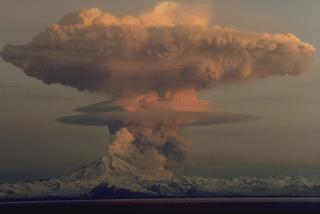
\includegraphics[width=0.3\paperwidth]{redoubt.jpg}$$
  \end{column}

  \begin{column}{0.33\paperwidth}
    $$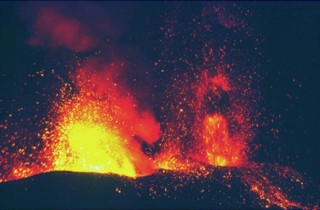
\includegraphics[width=0.3\paperwidth]{etna.jpg}$$
  \end{column}
  
\end{columns}
\vspace{-2cm}

\DeclareMathOperator\erf{erf}

\begin{document}

\begin{frame}
\titlepage % Print the title page as the first slide
\end{frame}

%\begin{frame}
%\frametitle{Overview} % Table of contents slide, comment this block out to remove it
%\tableofcontents % Throughout your presentation, if you choose to use \section{} and \subsection{} commands, these will automatically be printed on this slide as an overview of your presentation
%\end{frame}


%----------------------------------------------------------------------------------------
%	PRESENTATION SLIDES
%----------------------------------------------------------------------------------------

%------------------------------------------------
%\section{First Section} % Sections can be created in order to organize your presentation into discrete blocks, all sections and subsections are automatically printed in the table of contents as an overview of the talk
%------------------------------------------------

%\subsection{Subsection Example} % A subsection can be created just before a set of slides with a common theme to further break down your presentation into chunks

\begin{frame}
  \frametitle{Magma density}

  \begin{columns}[t]
    \begin{column}{0.45\paperwidth}
      \vspace{-1cm}

      $$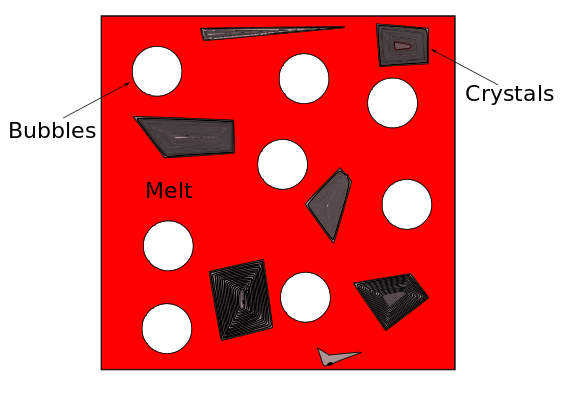
\includegraphics[width=0.3\paperwidth]{3_phase.png}$$
    \end{column}

    \begin{column}{0.45\paperwidth}
      Bulk density depends on volume fraction of crystals and bubbles

      \vspace{-0.5cm}

      $$ \rho = \rho_{\text{m}} \left(1 - \sum_{i} \phi_{i}\right) + \sum_{i} \rho_{i} \phi_{i} $$

    \end{column}

  \end{columns}

  \vspace{0.25cm}
  
  $\rho_{\text{m}}$ = Melt density \\
  \begin{itemize}
  \item Depends on $T, P, \mathbf{X}$ \\
  \end{itemize}

  \vspace{0.25cm}
  
  $i$ = quartz, hornblende, plagioclase etc. and H$_{2}$O, CO$_{2}$ bubbles etc.\\

  \vspace{0.25cm}
  
  $\rho_{i}$ = Density of phase $i$ \\
  \begin{itemize}
  \item Depends on $T, P$ for bubbles \\
  \item Depends on composition for crystals \\
  \end{itemize}

  \vspace{0.25cm}
  
  $\phi_{i}$ = Volume fraction of phase $i$ \\
    
  
\end{frame}
%------------------------------------------------

\begin{frame}
  \frametitle{Melt density}

  $$\rho_{m} = \sum_{i} X_{i} M_{i} \left(\sum_{i} X_{i} \bar{V_{i}}(T, P)\right)^{-1}$$

  $M_{i}$ = Molar mass of component $i$\\
  \begin{itemize}
  \item Mass of 1 mol of $i$ \\
  \item $M_{\text{SiO}_{2}} = 28$ g mol$^{-1}$ $+ 2 \times 16$ g mol$^{-1}$ = 60 g mol$^{-1}$\\
  \item $M_{\text{H}_{2}\text{O}} = 2 \times 1$ g mol$^{-1}$ $+ 16$ g mol$^{-1}$ = 18 g mol$^{-1}$\\
  \end{itemize}

  $\bar{V_{i}}$ = Partial molar volume of component $i$ \\
  \begin{itemize}
    \item Change in mixture volume when 1 mol of $i$ is added \\
  \end{itemize}

  Need to determine $\bar{V_{i}}(T, P)$ empirically \\
\end{frame}
%------------------------------------------------

\begin{frame}
  \frametitle{Melt density - Equation of state (EoS)}

  Relationship between \textbf{pressure}, \textbf{volume (density)} and \textbf{temperature} \\

  Experiments - measure volume of a sample of $\mathbf{X}$ at a different $P$ and $T$. \\

  Find \textbf{empirical} EoS

  \tiny $$ V_{m}(T, P, \mathbf{X}) = \sum_{i} X_{i} \left[ \textcolor{red}{\bar{V_{i}}(T = T_{\text{R}}, P = P_{\text{R}})} + \textcolor{blue}{\left. \frac{\partial \bar{V_{i}}(T, P = P_{\text{R}})}{\partial T}\right|_{T = T_{\text{R}}}} (T - T_{\text{R}}) + \textcolor{green}{\left.\frac{\partial \bar{V_{i}}(T = T_{\text{R}}, P)}{\partial P}\right|_{P = P_{R}}} (P - P_{\text{R}})\right]$$

  \begin{columns}[t]

    \begin{column}{0.3\paperwidth}

      $T_{\text{R}}$ = Reference temperature = 1673 K \\
      $P_{\text{R}}$ = Reference pressure = 10$^{-4}$ GPa \\

      \vspace{1cm}
      Lange \& Carmichael (1990) \\
      Lange (1997) \\
      Ochs \& Lange (1997)

    \end{column}

    \begin{column}{0.7\paperwidth}

      \begin{tabular}{|c|c|c|c|}
        \hline
        & $\textcolor{red}{\bar{V_{i}}(T = T_{\text{R}}, P = P_{\text{R}})}$ & $\textcolor{blue}{\left.\frac{\partial \bar{V_{i}}(T, P = P_{\text{R}})}{\partial T}\right|_{T = T_{\text{R}}}}$ & $\textcolor{green}{\left.\frac{\partial \bar{V_{i}}(T = T_{\text{R}}, P)}{\partial P}\right|_{P = P_{R}}}$ \\
        & /10$^{-6}$ m$^{3}$ mol$^{-1}$ & /10$^{-9}$ m$^{3}$ mol$^{-1}$ K & /10$^{-6}$ m$^{3}$ mol$^{-1}$ GPa \\
        \hline
        SiO$_{2}$ & 26.86 & 0.0 & -1.89 \\
        TiO$_{2}$ & 23.16 & 7.24 & -2.31 \\
        Al$_{2}$O$_{3}$ & 37.42 & 0.0 & -2.31 \\
        Fe$_{2}$O$_{3}$ & 42.13 & 9.09 & -2.53 \\
        FeO & 13.65 & 2.92 & -0.45 \\
        MgO & 11.69 & 3.27 & 0.27 \\
        CaO & 16.53 & 3.74 & 0.34 \\
        Na$_{2}$O & 28.88 & 7.68 & -2.40 \\
        K$_{2}$O & 45.07 & 12.08 & -6.75 \\
        Li$_{2}$O & 16.85 & 5.25 & -1.02 \\
        H$_{2}$O & 26.27 & 9.46 & -3.15 \\
        CO$_{2}$ & 33.0 & 0.0 & 0.0 \\
        \hline
        
      \end{tabular}
    \end{column}

  \end{columns}

\end{frame}
%------------------------------------------------
\begin{frame}
  \frametitle{Melt density - Effect of $T$ and $X_{\text{H}_{2}\text{O}}$}

  \vspace{-1cm}

  \begin{columns}[t]

    \begin{column}{0.45\paperwidth}

      $$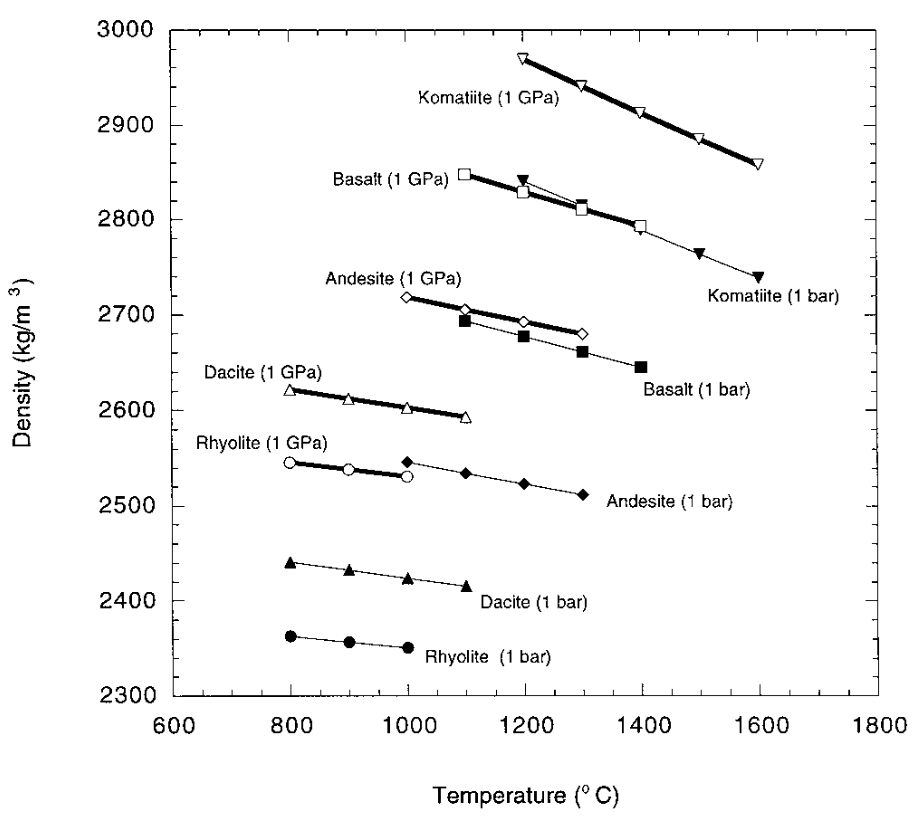
\includegraphics[width=\textwidth]{density_temp.png}$$

    \end{column}

    \begin{column}{0.45\paperwidth}

      $$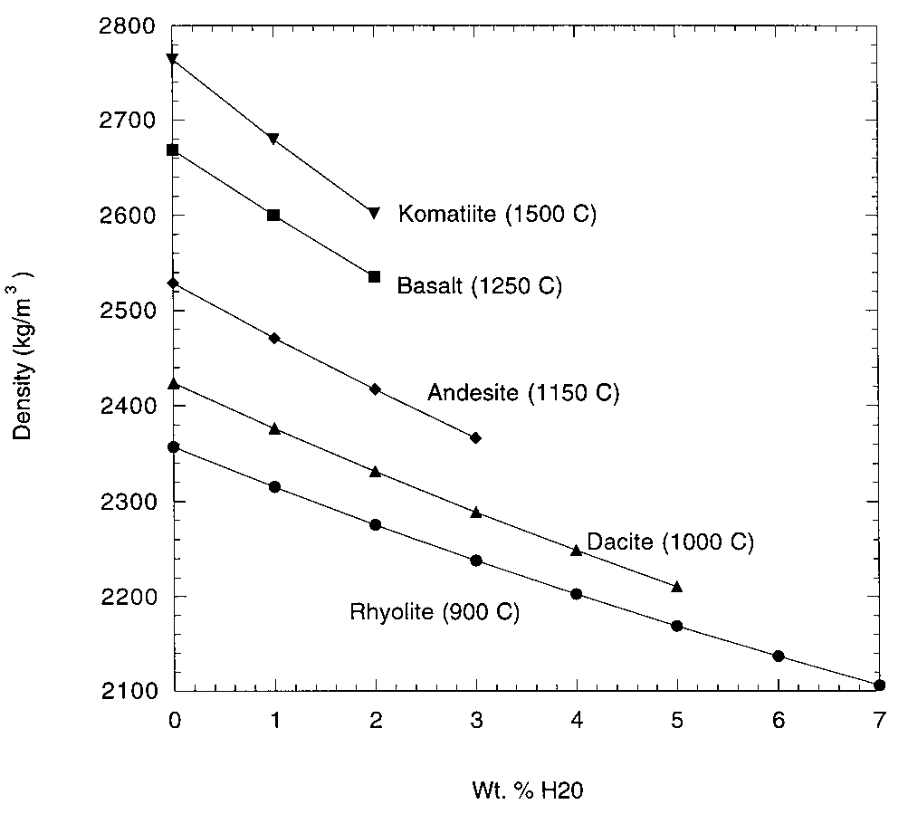
\includegraphics[width=\textwidth]{density_H2O.png}$$
      
    \end{column}

  \end{columns}

  Temperature has small effect on density, particularly for high-silica melts \\

  \vspace{1cm}
  
  Water content has much stronger effect \\
    
\end{frame}
%------------------------------------------------
\begin{frame}
  \frametitle{Magma viscosity - Viscosity definition}

  \textbf{Viscosity} - A measure of a substance's resistance to flow (deformation). It relates an applied shear stress to the velocity gradient. \\

  \begin{columns}[t]

    \begin{column}{0.45\paperwidth}

      $$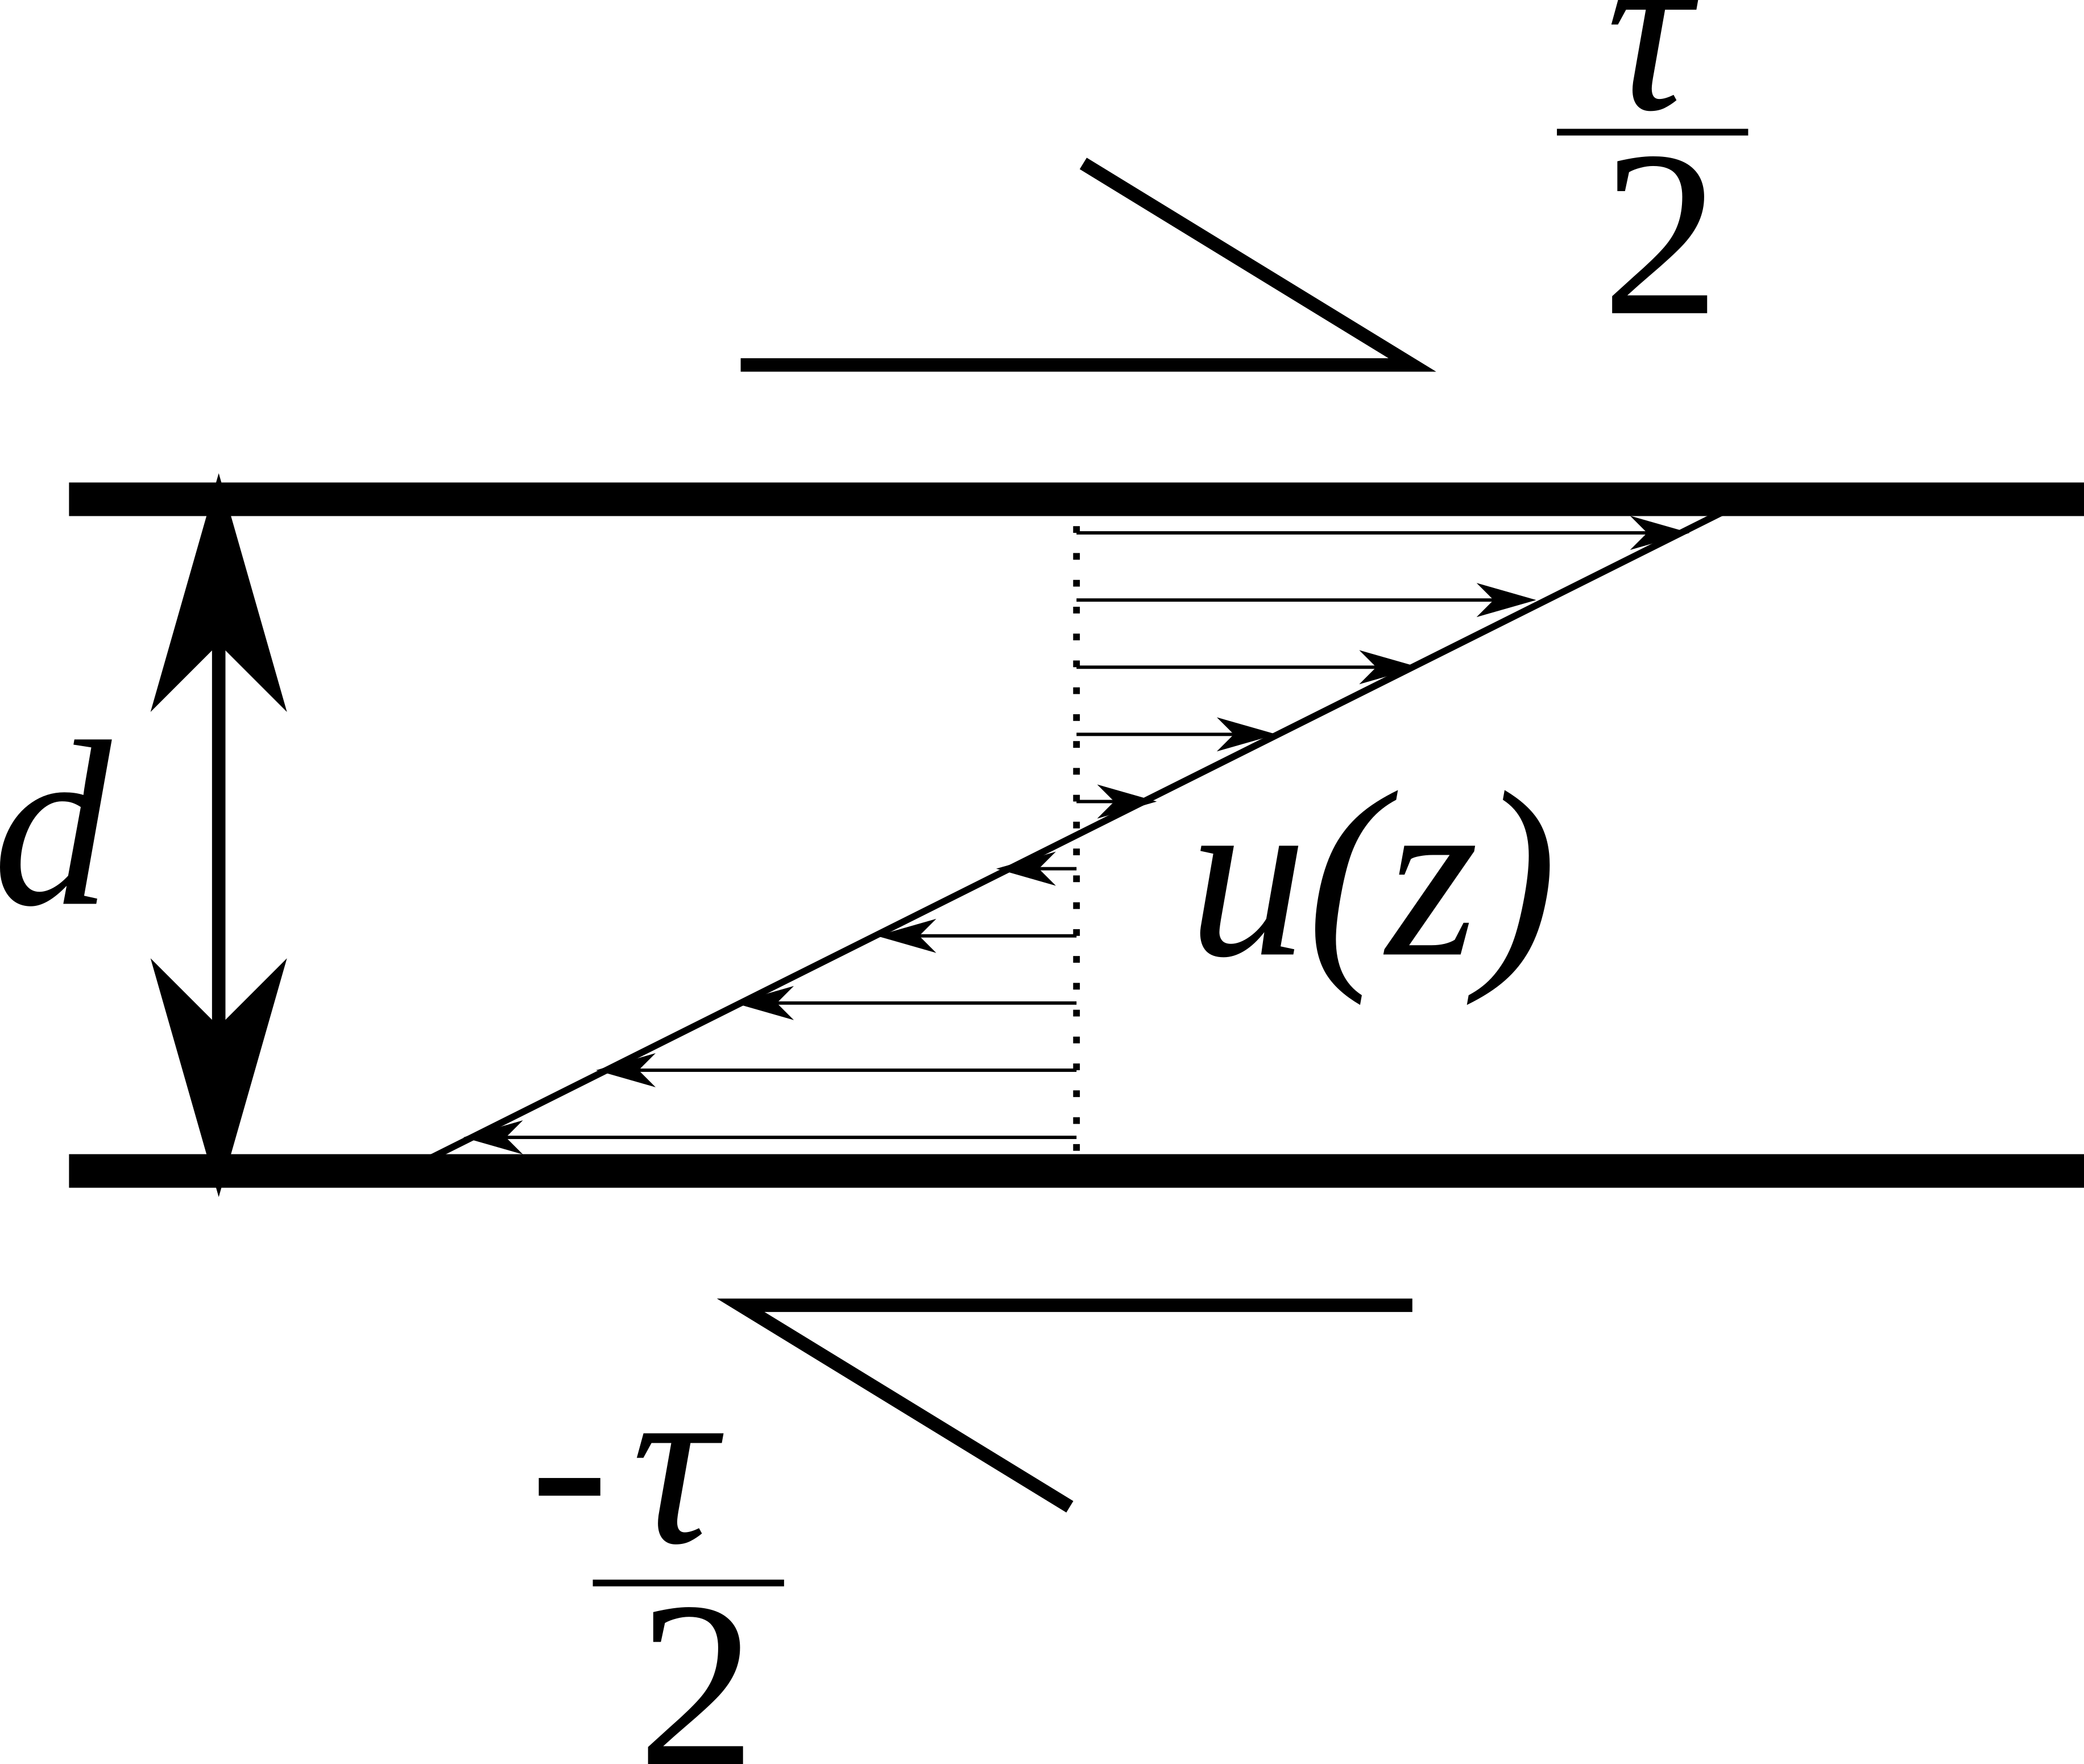
\includegraphics[width=\textwidth]{viscosity.png}$$

    \end{column}

    \begin{column}{0.45\paperwidth}

      Consider fluid between two sheared parallel plates\\

      \vspace{0.5cm}

      $\tau$ = Applied shear stress \\

      $d$ = Separation between plates \\

      $u(z)$ = Fluid velocity in gap \\

      \vspace{0.5cm}

      Viscosity $\eta$ is defined as:

      $$ \tau = \eta \frac{\mathrm{d} U}{\mathrm{d} z} = \eta \dot{\epsilon}$$

      where $\dot{\epsilon} = \mathrm{d} U / \mathrm{d} z$ = \textbf{strain rate}
    \end{column}

  \end{columns}
\end{frame}
%------------------------------------------------
\begin{frame}
  \frametitle{Magma viscosity - Newtonian fluids}

  Generally, viscosity is a function of strain rate: $\eta = \eta(\dot{\epsilon})$ \\

  \vspace{0.5cm}

  Therefore, impossible to assign a single value of $\eta$ to a material \\

  \vspace{0.5cm}

  \textbf{Newtonian fluids} - Special case where $\eta$ is independent of $\dot{\epsilon}$ \\

  \vspace{-1cm}
  
  \begin{columns}[t]

    \begin{column}{0.45\paperwidth}

      $$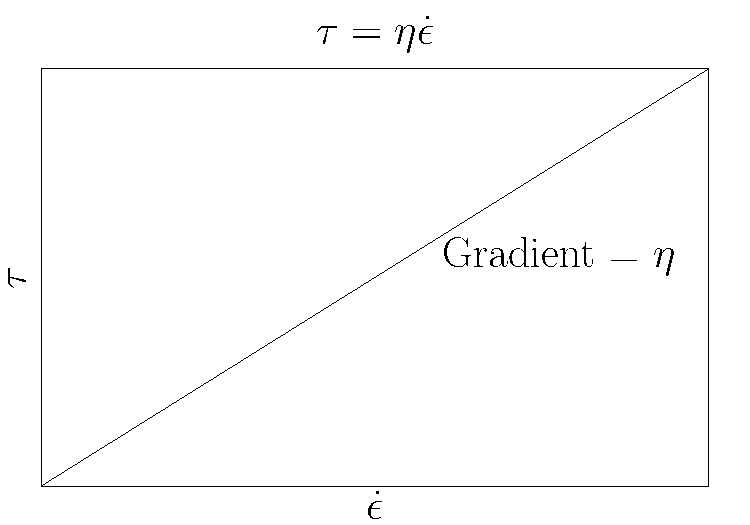
\includegraphics[width=\textwidth]{newtonian.pdf}$$

    \end{column}

    \begin{column}{0.45\paperwidth}

      \vspace{1cm}
      
      \textbf{Flow curve} - Relationship between $\tau$ and $\dot{\epsilon}$ \\

      $$ \tau = \eta(\dot{\epsilon}) \dot{\epsilon} $$

      \vspace{0.25cm}

      For Newtonian fluid, $\eta$ = constant \\

      \vspace{0.25cm}

      $\implies$ flow curve is straight line \\

      $\implies$ gradient = $\eta$ \\
      

    \end{column}

  \end{columns}

\end{frame}
%------------------------------------------------
\begin{frame}
  \frametitle{Magma viscosity - Rheological materials}

  \begin{columns}[t]

    \begin{column}{0.45\paperwidth}

      $$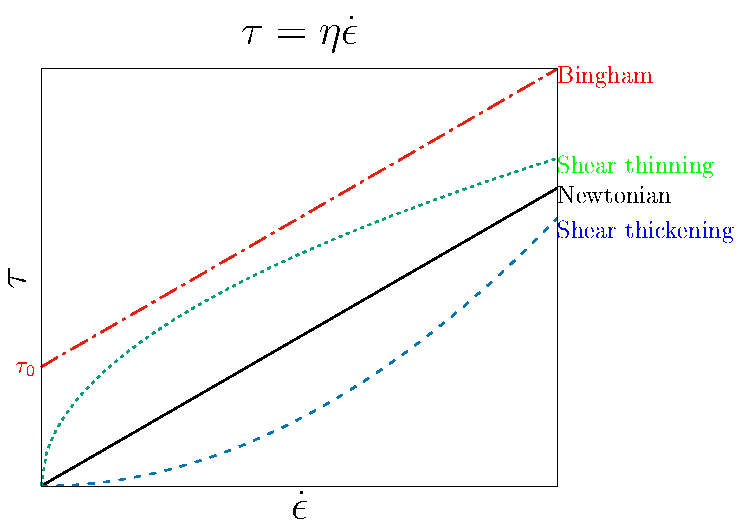
\includegraphics[width=\textwidth]{flow_curves.pdf}$$

    \end{column}

    \begin{column}{0.45\paperwidth}

      \vspace{-0.5cm}

      \textbf{Newtonian}
      \begin{itemize}
      \item Constant $\eta$ \\
      \item e.g. water, magmatic melt \\
      \end{itemize}

      \textbf{\textcolor{blue}{Shear thickening}}
      \begin{itemize}
      \item $\eta$ increases with $\dot{\epsilon}$ \\
      \item e.g. cornstarch \\
      \end{itemize}

      \textbf{\textcolor{green}{Shear thinning}}
      \begin{itemize}
      \item $\eta$ decreases with $\dot{\epsilon}$ \\
      \item e.g. butter \\
      \end{itemize}

      \textbf{\textcolor{red}{Bingham}}
      \begin{itemize}
      \item Fluid has \textbf{yield stress} $\tau_{0}$ \\
      \item For $\tau < \tau_{0}$ fluid does not flow ($\dot{\epsilon} = 0$) \\
      \item e.g. Mayonaise
      \end{itemize}
      
\end{column}

  \end{columns}

\end{frame}
%------------------------------------------------
\begin{frame}
  \frametitle{Measuring rheological properties}

  \begin{columns}[t]

    \begin{column}{0.33\paperwidth}

      \centering Parallel plate
      
      $$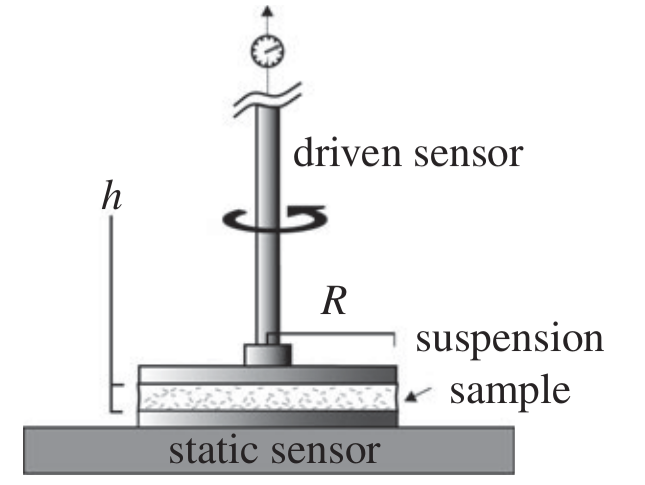
\includegraphics[width=\textwidth]{parallelPlate.png}$$

    \end{column}

    \begin{column}{0.33\paperwidth}

      \centering Cone and plate
      
      $$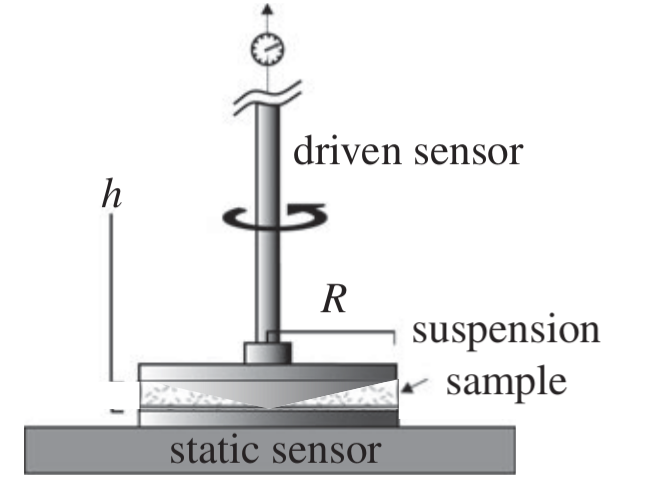
\includegraphics[width=\textwidth]{conePlate.png}$$

    \end{column}

    \begin{column}{0.33\paperwidth}

      \centering Concentric cylinder
      
      $$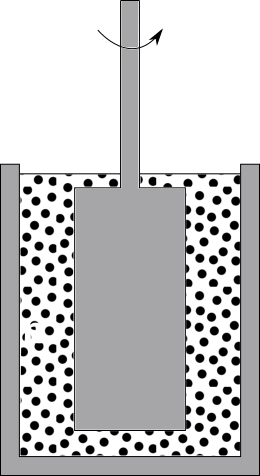
\includegraphics[width=0.5\textwidth]{concentricCylinder.png}$$

    \end{column}
    
  \end{columns}

  Apply torque $M \implies$ stress $\tau$ \\
  Measure angular velocity $\Omega \implies$ strain rate $\dot{\gamma}$ \\
  Determine flow curve $\tau = \eta(\dot{\gamma}) \dot{\gamma}$
\end{frame}
%------------------------------------------------
\begin{frame}
  \frametitle{Magma viscosity - Melt as a Newtonian fluid}

  Silica melt is almost perfectly Newtonian. \\

  \vspace{0.5cm}

  However, at extremely high shear rates, all materials start to undergo shear-thinning \\

  \vspace{0.5cm}

  Critical shear rate is given by

  $$ \dot{\epsilon_{c}} \approx \frac{10^{-3} G}{\eta_{m}} $$

  $G$ = Shear modulus $\approx 10^{10}$ Pa

  \vspace{0.5cm}

  At even higher shear rates, the melt cannot deform as a fluid and snaps in a brittle manner. 
\end{frame}
%------------------------------------------------
\begin{frame}
  \frametitle{Magma viscosity - Melt viscosity}


  Melt is modelled according to the Vogel-Fulchner-Tammann (VFT) equation (Giordano et al., 2008)\\

  \begin{columns}[t]

    \begin{column}{0.5\textwidth}

      $$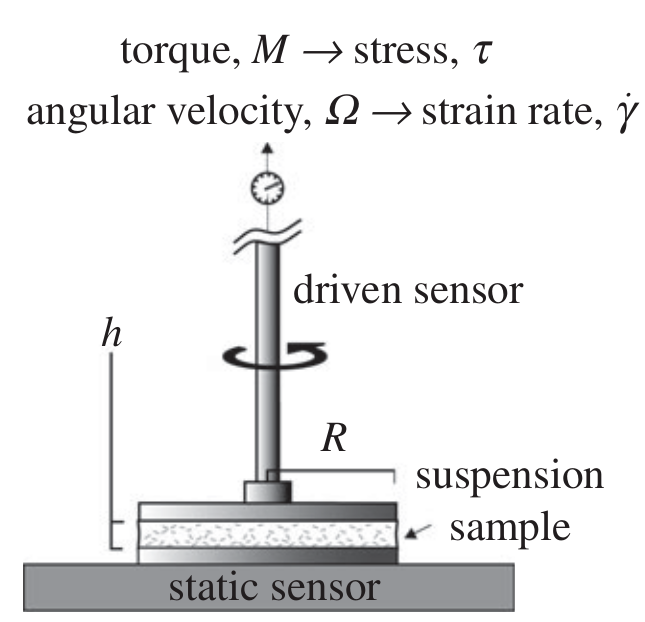
\includegraphics[width=\textwidth]{rheometer.png}$$

    \end{column}

    \begin{column}{0.5\textwidth}

      $$ \log \eta_{\text{m}} = A + \frac{B(\mathbf{X})}{T - C(\mathbf{X})}$$

      $$\eta_{\text{m}} = 10 ^{A + B(\mathbf{X})/[T - C(\mathbf{X})]}$$

      \small Measurements of the viscosity of samples of different $\mathbf{X}$ at different $T$ are used to determine $A, B(\mathbf{X}), C(\mathbf{X})$ \\

      \vspace{0.5cm}

      N.B: This is a fitted, purely empirical equation - it is not dimensionally consistent!
      
    \end{column}

  \end{columns}
  

\end{frame}
%------------------------------------------------
\begin{frame}
  \frametitle{Magma viscosity - Fitted parameters}

  \begin{columns}[t]

    \begin{column}{0.5\paperwidth}

      \centering
      
      $A$ = constant = -4.55
      
      \vspace{0.5cm}

      $B = \sum_{i = 1}^{7} b_{i} M_{i} + \sum_{j = 1}^{3} b_{1j} M_{1j}$ 

      \vspace{0.5cm}

      $C = \sum_{i = 1}^{6} c_{i} N_{i} + c_{11} N_{11}$

      \vspace{1cm}

    \end{column}

    \begin{column}{0.5\paperwidth}

      $$ \log \eta_{\text{m}} = A + \frac{B(\mathbf{X})}{T - C(\mathbf{X})}$$

      $$\eta_{\text{m}} = 10 ^{A + B(\mathbf{X})/[T - C(\mathbf{X})]}$$

    \end{column}

  \end{columns}
  
  \tiny
  \begin{tabular}{|c|c||c|c|}
    \hline
    $b_{1} = 159.6$ & $M_{1} = X_{\text{SiO}_{2}} + X_{\text{TiO}_{2}}$ & $c_{1} = 2.75$ & $N_{1} = X_{SiO_{2}}$ \\
    $b_{2} = -173.3$ & $M_{2} = X_{\text{Al}_{2}\text{O}_{3}}$ & $c_{2} = 15.7$ & $N_{2} = X_{\text{TiO}_{2}} + X_{\text{Al}_{2}\text{O}_{3}}$ \\
    $b_{3} = -72.1$ & $M_{3} = X_{\text{FeO}} + X_{\text{MnO}} + X_{\text{P}_{2}\text{O}_{5}}$ & $c_{3} = 8.3$ & $N_{3} = X_{\text{FeO}} + X_{\text{MnO}} + X_{\text{MgO}}$ \\
    $b_{4} = -75.7$ & $M_{4} = X_{\text{MgO}}$ & $c_{4} = 10.2$ & $N_{4} = X_{\text{CaO}}$ \\
    $b_{5} = -39.9$ & $M_{5} = X_{\text{CaO}}$ & $c_{5} = -12.3$ & $N_{5} = X_{\text{Na}_{2}\text{O}} + X_{\text{K}_{2}\text{O}}$ \\
    $b_{6} = -84.1$ & $M_{6} = X_{\text{Na}_{2}\text{O}} + X_{\text{H}_{2}\text{O}} + X_{\text{F}_{2}\text{O}}$ & $c_{6} = -99.1$ & $N_{6} = \ln(1 + X_{\text{H}_{2}\text{O}} + X_{\text{F}_{2}\text{O}})$ \\
    $b_{7} = -141.5$ & $M_{7} = X_{\text{H}_{2}\text{O}} + X_{\text{F}_{2}\text{O}} + \ln(1 + X_{\text{H}_{2}\text{O}})$& &  \\
    \hline
    $b_{11} = -2.43$ & $M_{11} = M_{1} N_{3}$ & $c_{11} = 0.3$& $N_{11} = (M_{2} + N_{3} + N_{4} - $\\
    $b_{12} = -0.91$ & $M_{12} = (N_{1} + N_{2} + X_{\text{P}_{2}\text{O}_{5}}) (N_{5} + X_{\text{H}_{2}\text{O}})$ & & $X_{\text{P}_{2}\text{O}_{5}}) (N_{5} + X_{\text{H}_{2}\text{O}} + X_{\text{F}_{2}\text{O}_{-1}})$ \\
    $b_{13} = 17.6$ & $M_{13} = M_{2} N_{5}$ & &  \\    
    \hline
  \end{tabular}

  \vspace{0.5cm}

  \normalsize For a given melt composition, can evaluate $\eta$ \\
  
\end{frame}
%------------------------------------------------
\begin{frame}
  \frametitle{Melt viscosity - Effect of $T$ and $X_{\text{H}_{2}\text{O}}$}

  \vspace{-1cm}

  \begin{columns}[t]

    \begin{column}{0.45\paperwidth}

      $$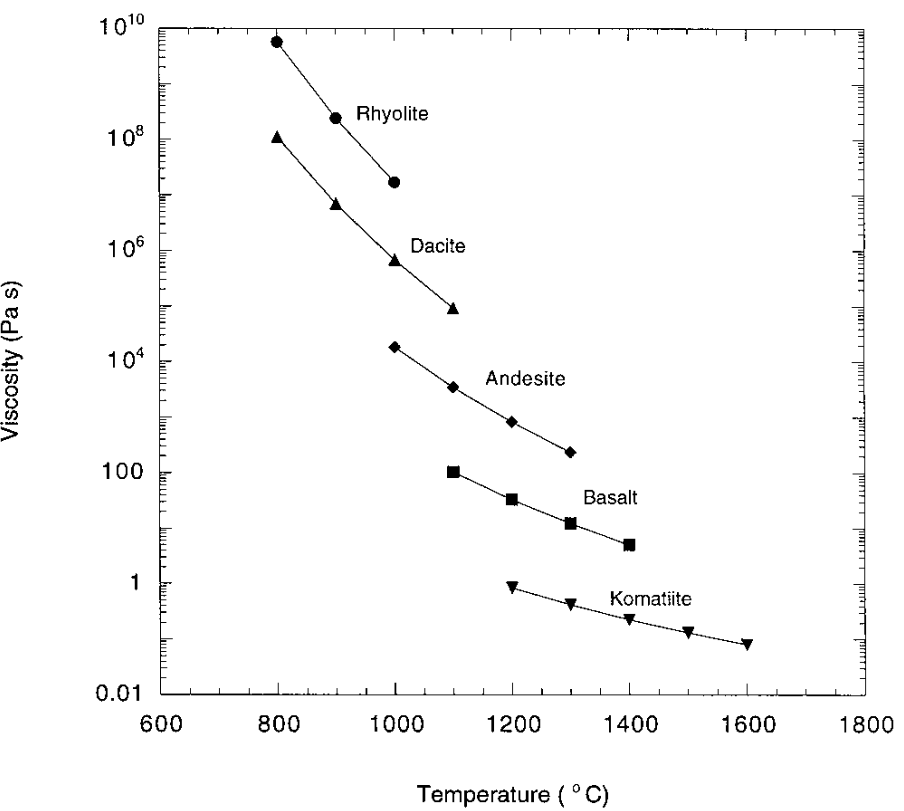
\includegraphics[width=\textwidth]{viscosity_temp.png}$$

    \end{column}

    \begin{column}{0.45\paperwidth}

      $$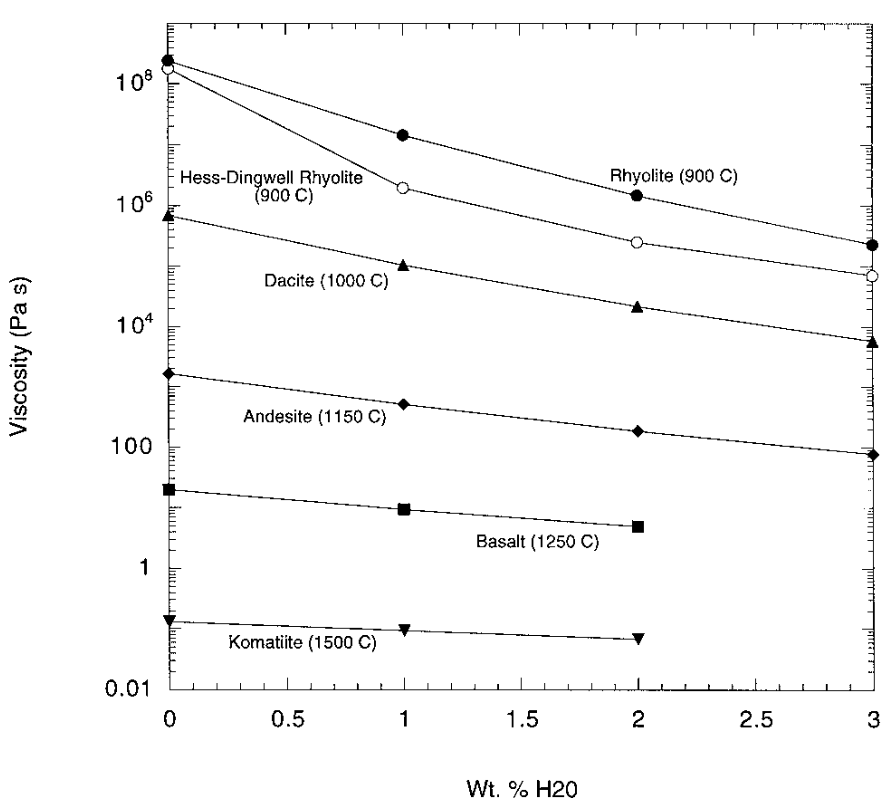
\includegraphics[width=\textwidth]{viscosity_H2O.png}$$
      
    \end{column}

  \end{columns}

  Increase in $T$ and $X_{\text{H}_{2}\text{O}}$ can reduce melt viscosity by orders of magnitude \\
    
\end{frame}
%------------------------------------------------
\begin{frame}
  \frametitle{Magma viscosity - Effect of crystals}

  Particles suspended in a fluid increase the viscosity of the medium \\

  \textbf{Suspension} - A mixture of particles and fluid \\

  $\phi_{\text{c}} = $ \textbf{Volume fraction} of crystals \\

  Define \textbf{relative viscosity} $\eta_{\text{r}}(\phi_{\text{c}})$ to contain effect of $\phi_{\text{c}}$

  $$ \eta = \eta_{\text{m}} \eta_{\text{r}}(\phi_{\text{c}}) $$

  \vspace{0.5cm}
  
  \begin{columns}[t]

    \begin{column}{0.5\textwidth}

      $\phi_{\text{c}} \lesssim 0.01$ - \textbf{Dilute} \\

      \vspace{0.5cm}
      
      $0.01 \lesssim \phi_{\text{c}} \lesssim 0.25$ - \textbf{Semi-dilute} \\

      \vspace{0.5cm}
      
      $\phi_{\text{c}} \gtrsim 0.25$ - \textbf{Concentrated} \\

    \end{column}

    \begin{column}{0.5\textwidth}

      \vspace{-1.5cm}
      
      $$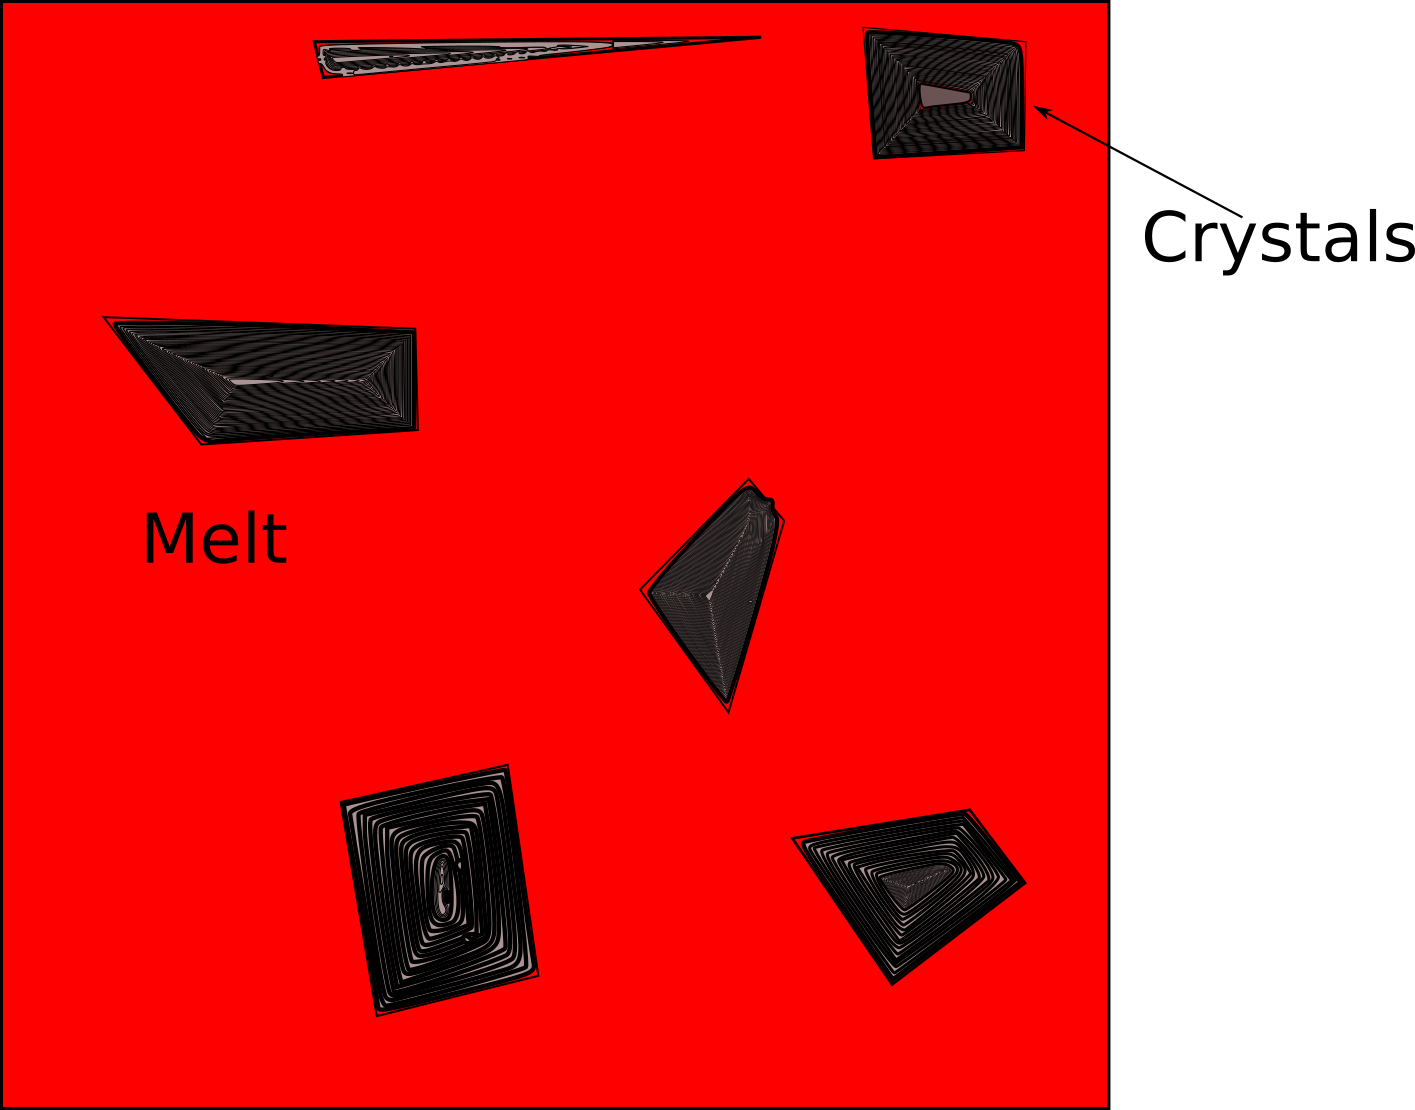
\includegraphics[width=\textwidth]{2_phase.png}$$

    \end{column}

  \end{columns}
  
  \end{frame}
%------------------------------------------------
\begin{frame}
  \frametitle{Magma viscosity - Dilute particle suspensions}

  \footnotesize \textbf{Dilute suspension}: $\phi_{\text{c}} \lesssim 0.01$ \\

  \vspace{0.5cm}

  Interactions between particles are weak and effect on viscosity is small \\

  \vspace{0.5cm}

  Viscosity depends linearly on $\phi_{\text{c}}$ (Einstein, 1906; 1911) \\

  \vspace{0.5cm}

  $$ \eta_{\text{r}} = 1 + B \phi_{\text{c}} $$ \\

  \vspace{0.5cm}

  Experiments suggest that $B \approx 2.5$ \\

  \vspace{0.5cm}

  Suspension rheology models are only strictly valid for suspensions on \textbf{spherical} particles. \\

  \vspace{0.5cm}

  Developing models for suspensions of differently shaped particles is difficult \\
  \hspace*{1cm} - particularly for magmas where crystals have many different and irregular shapes \\

  \vspace{0.5cm}

  However, for dilute and semi-dilute suspensions, models work well. \\
  
  \end{frame}
%------------------------------------------------
\begin{frame}
  \frametitle{Magma viscosity - Semi-dilute suspensions}

  \footnotesize \textbf{Semi-dilute suspension}: $0.01 \lesssim \phi_{\text{c}} \lesssim 0.25$ \\

  \vspace{0.5cm}

  Particles interact with each other, affecting the viscosity \\

  \vspace{0.5cm}

  Viscosity depends non-linearly on $\phi_{\text{c}}$ (Guth \& Gold, 1938; Vand, 1948; Manley \& Mason, 1955) \\

  \vspace{0.5cm}

  Can model the viscosity with a \textbf{polynomial} expression \\

  \vspace{0.5cm}

  $$ \eta_{\text{r}} = 1 + B \phi_{\text{c}} + B_{1} \phi_{\text{c}}^{2} + ... $$ \\

  \vspace{0.5cm}

  Experiments suggest that $7.35 \lesssim B_{1} \lesssim 14.1$ \\

  \vspace{0.5cm}

  Predictions from polynomial models get worse as $\phi_{\text{c}}$ increases. \\
  \hspace*{1cm} - This is because as particles begin to touch the viscosity rises very fast \\

  
  \end{frame}
%------------------------------------------------
\begin{frame}
  \frametitle{Magma viscosity - Maximum packings}

  \footnotesize \textbf{Concentrated suspension}: $\phi_{\text{c}} \gtrsim 0.25$ \\

  \vspace{0.5cm}

  \textbf{Random close packing} - Maximum volume fraction of crystals that can be obtained in a disordered system \\
  \hspace*{1cm} For spheres: $\phi_{\text{m}} \approx 0.64$

  \textbf{Densest regular packing} - Maximum possible packing if crystals are arranged orderly 
  \hspace*{1cm} For spheres: $\phi_{\text{r}} \approx 0.74$

  \vspace{-1cm}
  
  \begin{columns}[t]

    \begin{column}{0.5\textwidth}

      $$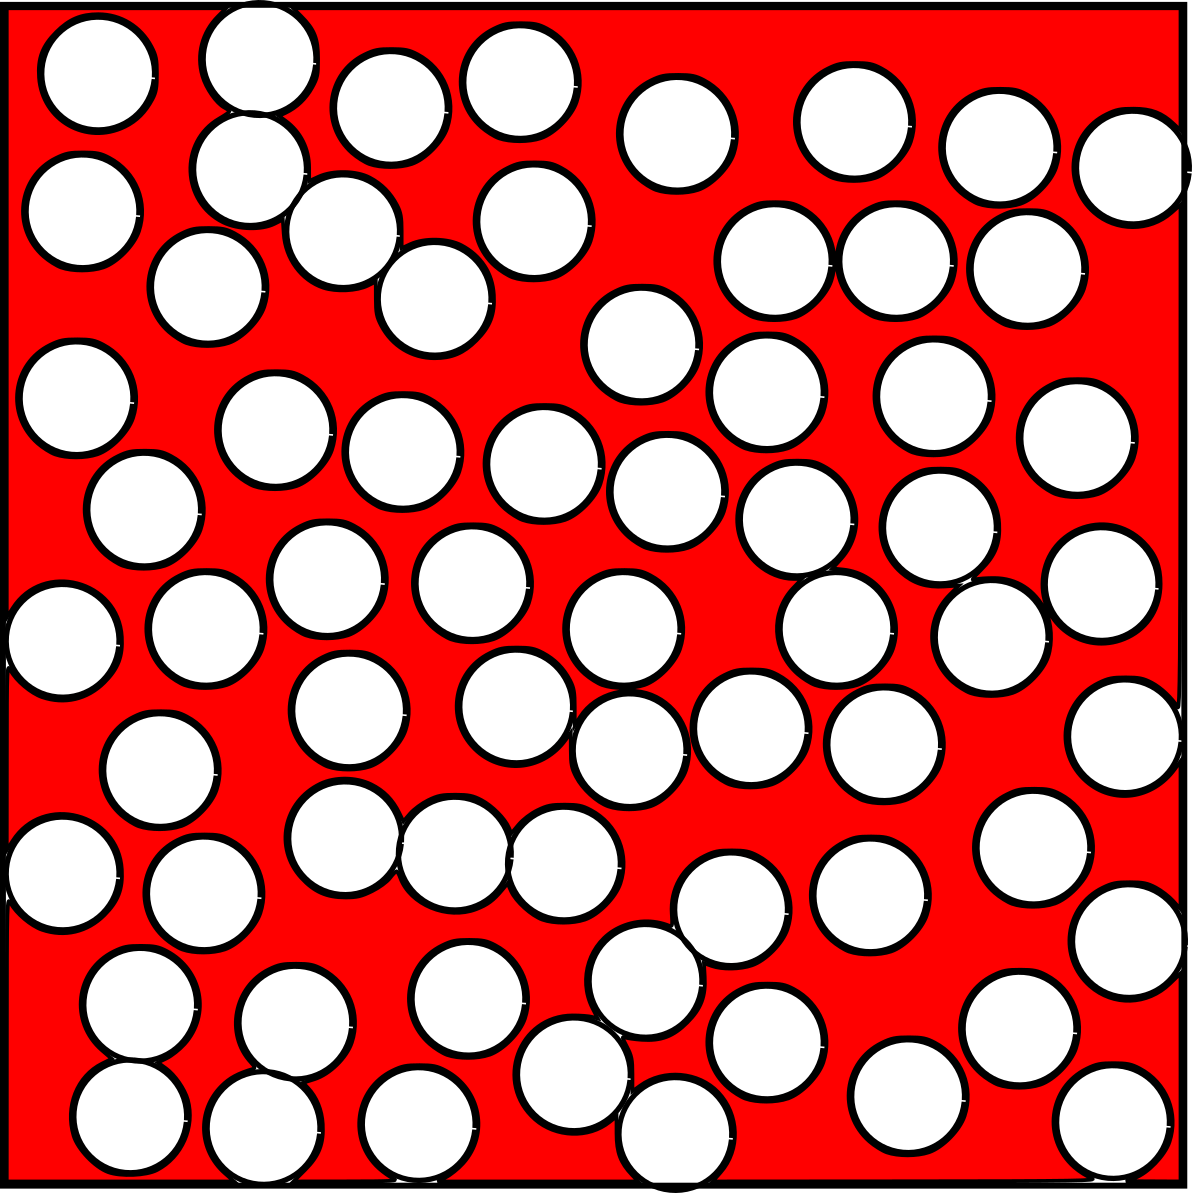
\includegraphics[width=0.8\textwidth]{random_close_packing.png}$$
      
    \end{column}

    \begin{column}{0.5\textwidth}

      $$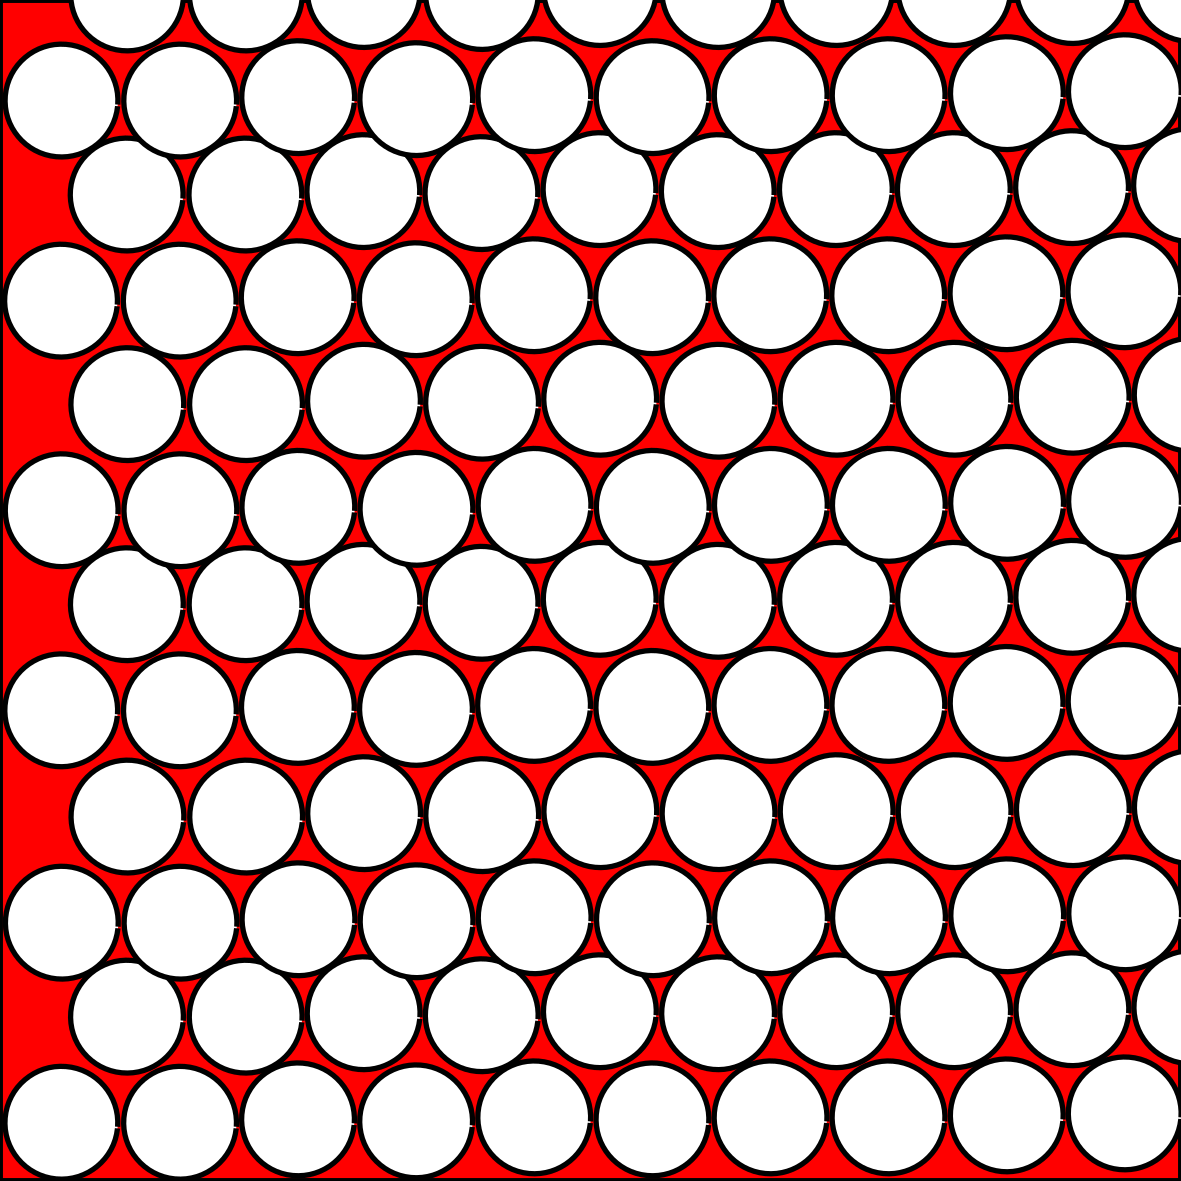
\includegraphics[width=0.8\textwidth]{densest_regular_packing.png}$$

    \end{column}
    
  \end{columns}
  
  \end{frame}
%------------------------------------------------
\begin{frame}
  \frametitle{Magma viscosity - Concentrated suspensions}

  \footnotesize \textbf{Concentrated suspension}: $\phi_{\text{c}} \gtrsim 0.25$ \\

  \vspace{0.5cm}

  Once $\phi_{\text{c}} = \phi_{\text{m}}$, then further deformation is impossible \\
  \hspace*{1cm} - the material is \textbf{rheologically locked} \\
  \hspace*{1cm} - $\eta_{\text{r}} \to \infty$ \\

  \vspace{0.5cm}
  
  For magmas, $\phi_{\text{m}}$ depends on crystal shape and size distribution \\
  \hspace*{1cm} - Very difficult to accurately predict \\
  \hspace*{1cm} - Many experiments, find $\phi_{\text{m}} \approx 0.4$ \\

  \vspace{0.5cm}

  Multiple models describe rheology of concentrated suspensions, but commonly used model is \textbf{Krieger \& Dougherty (1959)}

  $$ \eta_{\text{r}} = \left(1 - \frac{\phi_{\text{c}}}{\phi_{\text{m}}}\right)^{-B \phi_{\text{m}}}$$
\end{frame}
%------------------------------------------------
\begin{frame}
  \frametitle{Magma viscosity - Yield stress}

  Once a touching network of crystals exists, then the magma has a \textbf{yield stress}  
  \begin{columns}[t]

    \begin{column}{0.5\textwidth}

      $$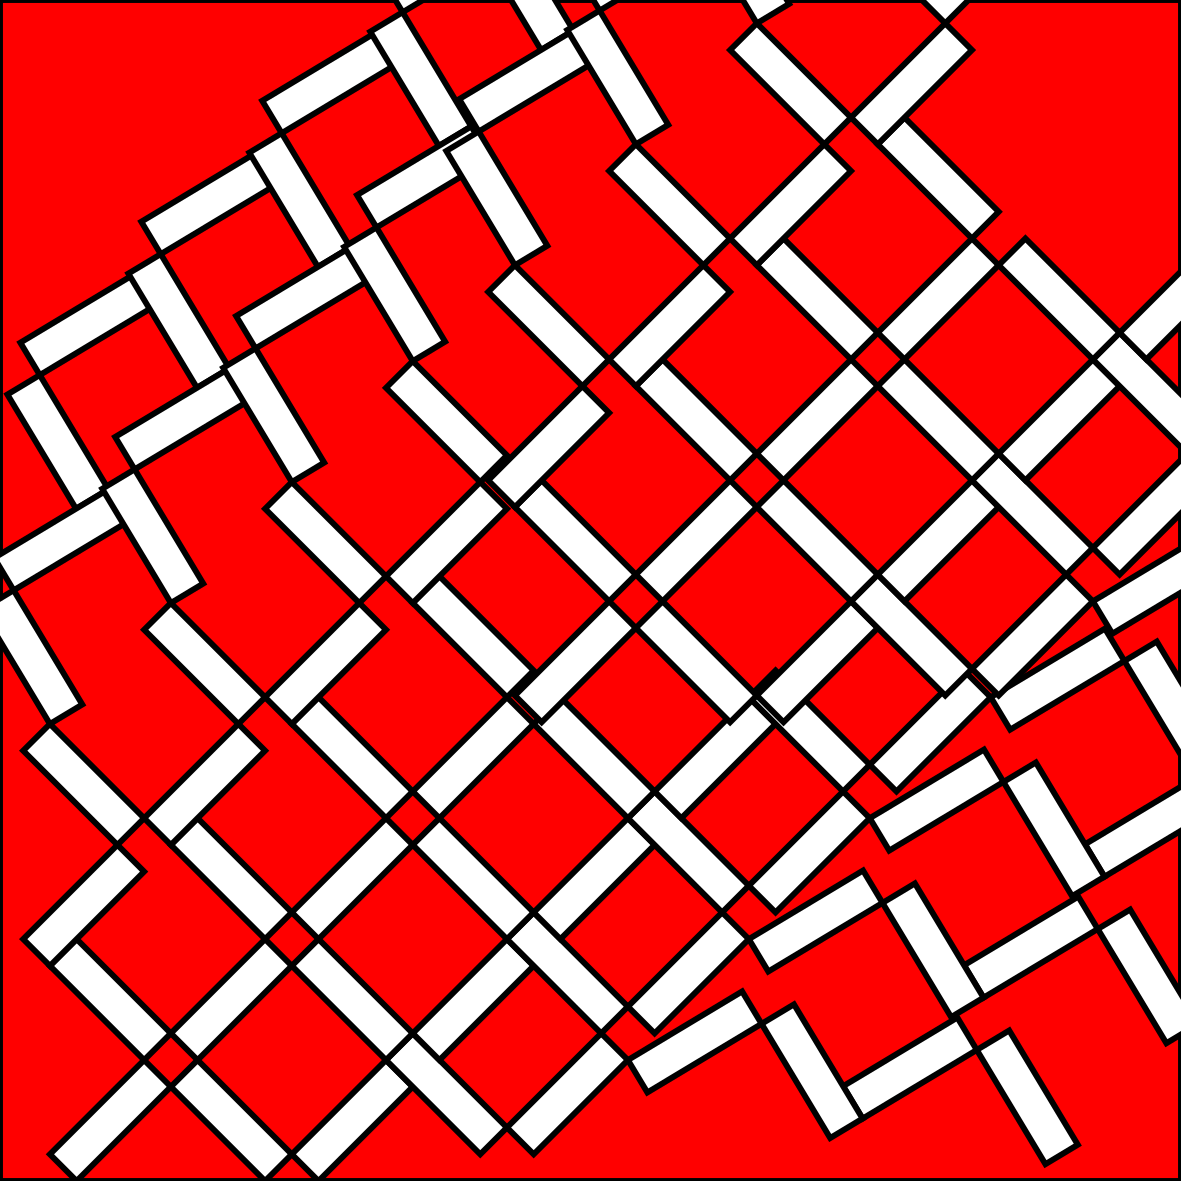
\includegraphics[width=0.8\textwidth]{crystal_network.png}$$
      
    \end{column}

    \begin{column}{0.5\textwidth}

      Experiments show magmas with $\phi_{\text{c}}$ as small as 0.2 can have a yield stress 

      \vspace{1cm}
      
      $\phi_{\text{y}} = $ Minimum value of $\phi_{\text{c}}$ at which yield stress exists

      $$ \tau_{0} = 6.9 \left( \frac{\phi_{\text{c}}}{\phi_{\text{y}}} - 1\right) \left(1 - \frac{\phi_{\text{c}}}{\phi_{\text{m}}}\right)^{-1}$$

      (Saar et al., 2001; Andrews \& Manga, 2014)
    \end{column}
    
  \end{columns}
\end{frame}
%------------------------------------------------
\begin{frame}
  \frametitle{Magma viscosity - Non-Newtonian effects}

  \footnotesize Definition of $\eta_{\text{r}}$ assumes Newtonian or Bingham rheology \\
  \hspace*{1cm} i.e. $\eta$ is independent of $\dot{\epsilon}$ \\

  \vspace{0.5cm}
  
  In reality:

  \begin{columns}[t]

    \begin{column}{0.5\textwidth}

      \vspace{-0.5cm}
      
      $$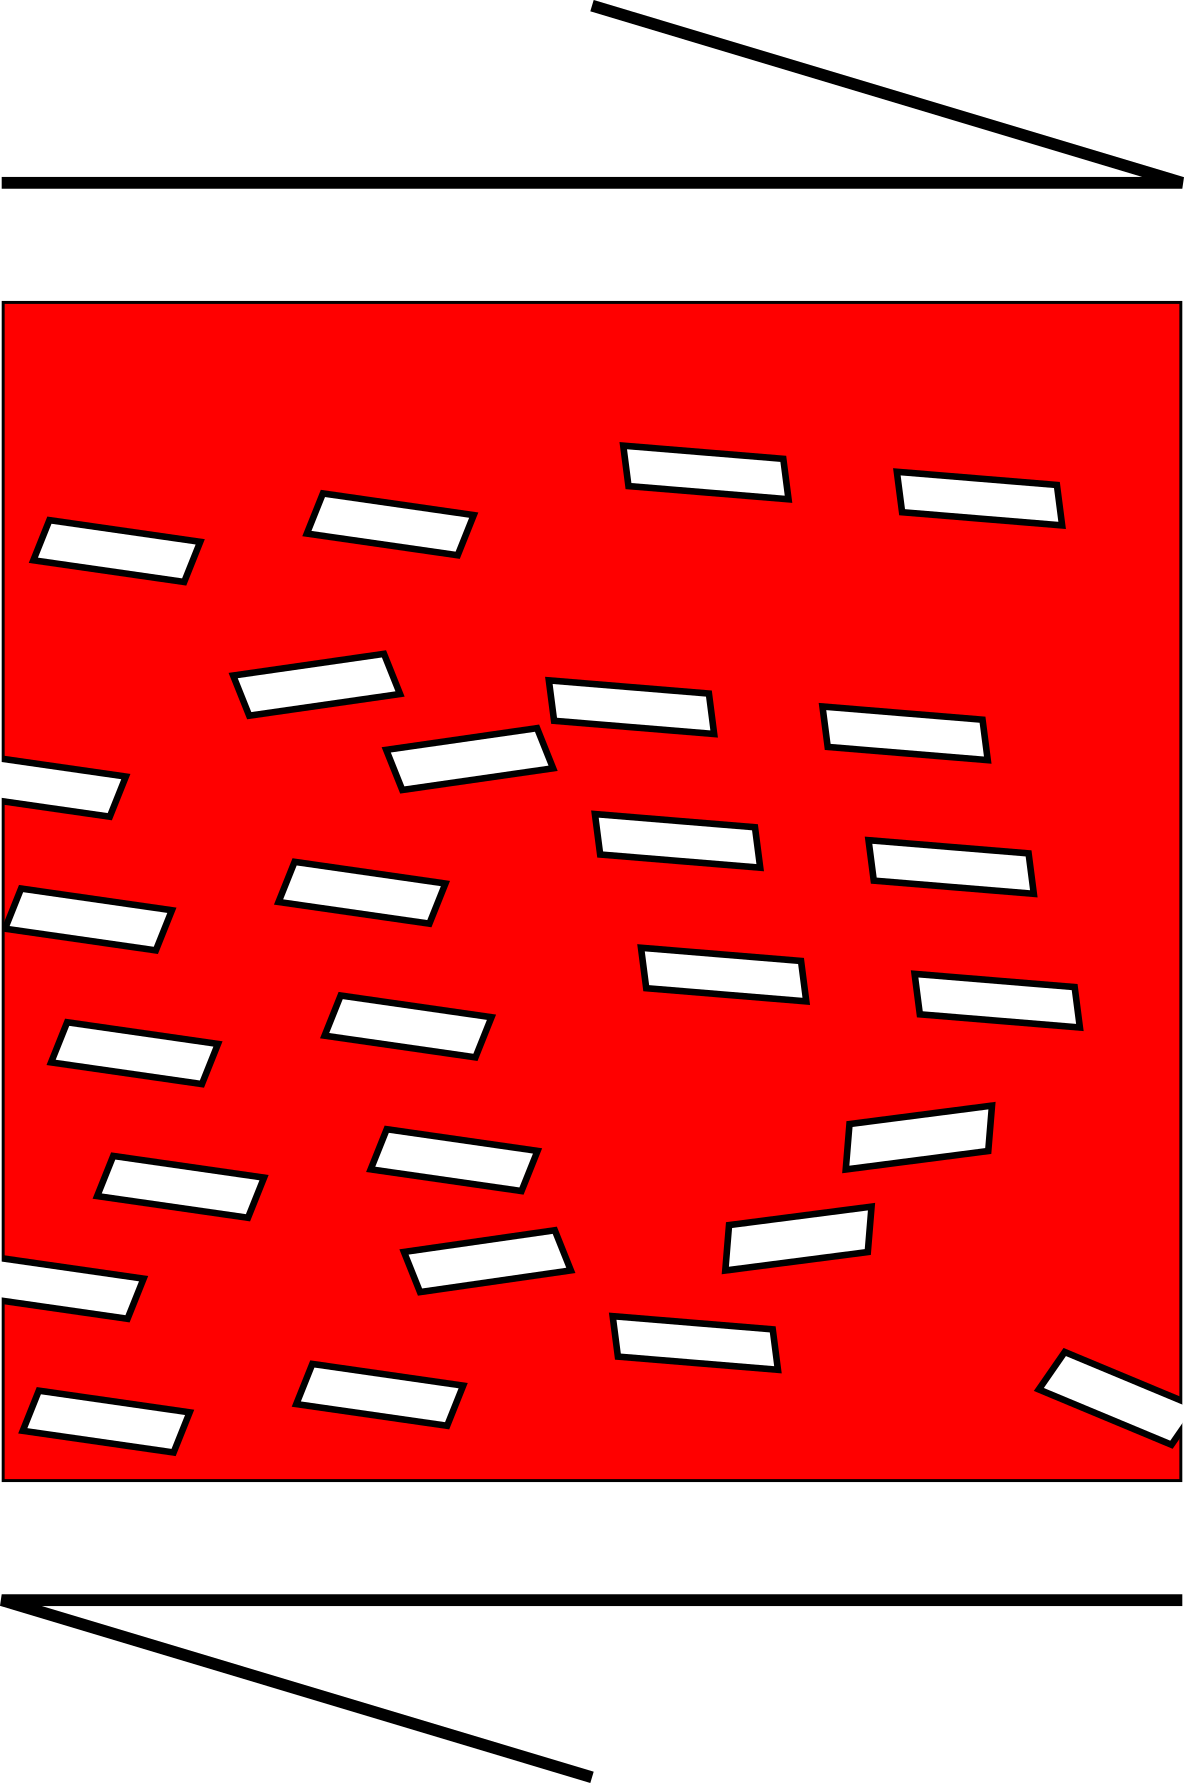
\includegraphics[width=0.65\textwidth]{flow_alignment.png}$$

    \end{column}
 
   \begin{column}{0.5\textwidth}

     Elongated particles align with the flow \\

     \vspace{0.5cm}
  
     Longest axis becomes parallel to flow lines \\

     \vspace{0.5cm}
  
     The greater the strain rate the larger the reduction in viscosity $\implies$ \textbf{shear thinning} \\

     \vspace{0.5cm}
  
     More complicated models exist to describe suspensions of elongate particles e.g. \\

     $$ \eta_{\text{r}} = \left(1 - \frac{\phi_{\text{c}}}{\phi_{\text{m}}}\right)^{-2} \dot{\epsilon}^{0.2 r_{\text{p}} (\phi_{\text{c}} / \phi_{\text{m}})^{4}} $$

     \vspace{0.2cm}
     
     $r_{\text{p}}$ = Crystal \textbf{aspect ratio} \\
    \end{column}

  \end{columns}
\end{frame}
%------------------------------------------------
\begin{frame}
  \frametitle{Magma rheology - Suspension or granular media}

  Classically, model mixtures of particles and fluid as \textbf{suspensions}:
  \begin{itemize}
  \item No relative motion between fluid and particles \\
  \item $\phi$ is control variable \\
  \item System described by equations of \textbf{fluid dynamics} with \textbf{effective viscosity} \\
  \end{itemize}

  In reality, particularly for dense suspensions:
  \begin{itemize}
  \item \textbf{Phase segregation} can be important \\
  \item $\phi$ can depend on particle pressure $P_{\text{p}}$ \\
  \item System is described by \textbf{Granular mechanics} with \textbf{interstitial fluid} \\
  \end{itemize}

  \begin{columns}[t]

    \begin{column}{0.5\paperwidth}

      $$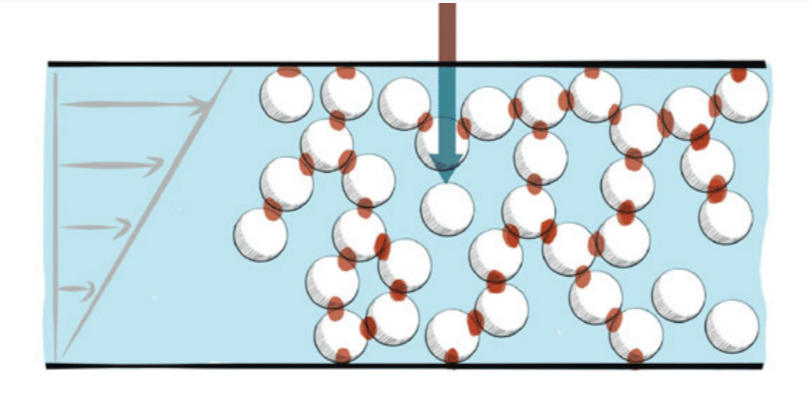
\includegraphics[width=0.65\textwidth]{Guazzelli18.png}$$

      \vspace{-0.2cm}

      \tiny \centering Guazzelli and Pouliquen (2018)
      
    \end{column}

    \begin{column}{0.5\paperwidth}

      How to describe these systems remains highly contentious \\

      Extremely difficult to model theoretically, numerically or experimentally \\

    \end{column}

  \end{columns}
  
\end{frame}
%------------------------------------------------
\begin{frame}
  \frametitle{Magma viscosity - Effect of bubbles}

  \footnotesize Rheological behaviour is determined by the \textbf{capillary} number \\

  $$ \text{Ca} = \frac{\eta_{\text{m}} \dot{\epsilon} r_{\text{b}}}{\sigma}$$

  \begin{columns}[t]

    \begin{column}{0.5\textwidth}

      $\eta_{\text{m}}$ = Melt viscosity \\
      
      $\dot{\epsilon}$ = Shear rate \\

      $r_{\text{b}}$ = Bubble radius \\

      $\sigma$ = Surface tension \\

      $$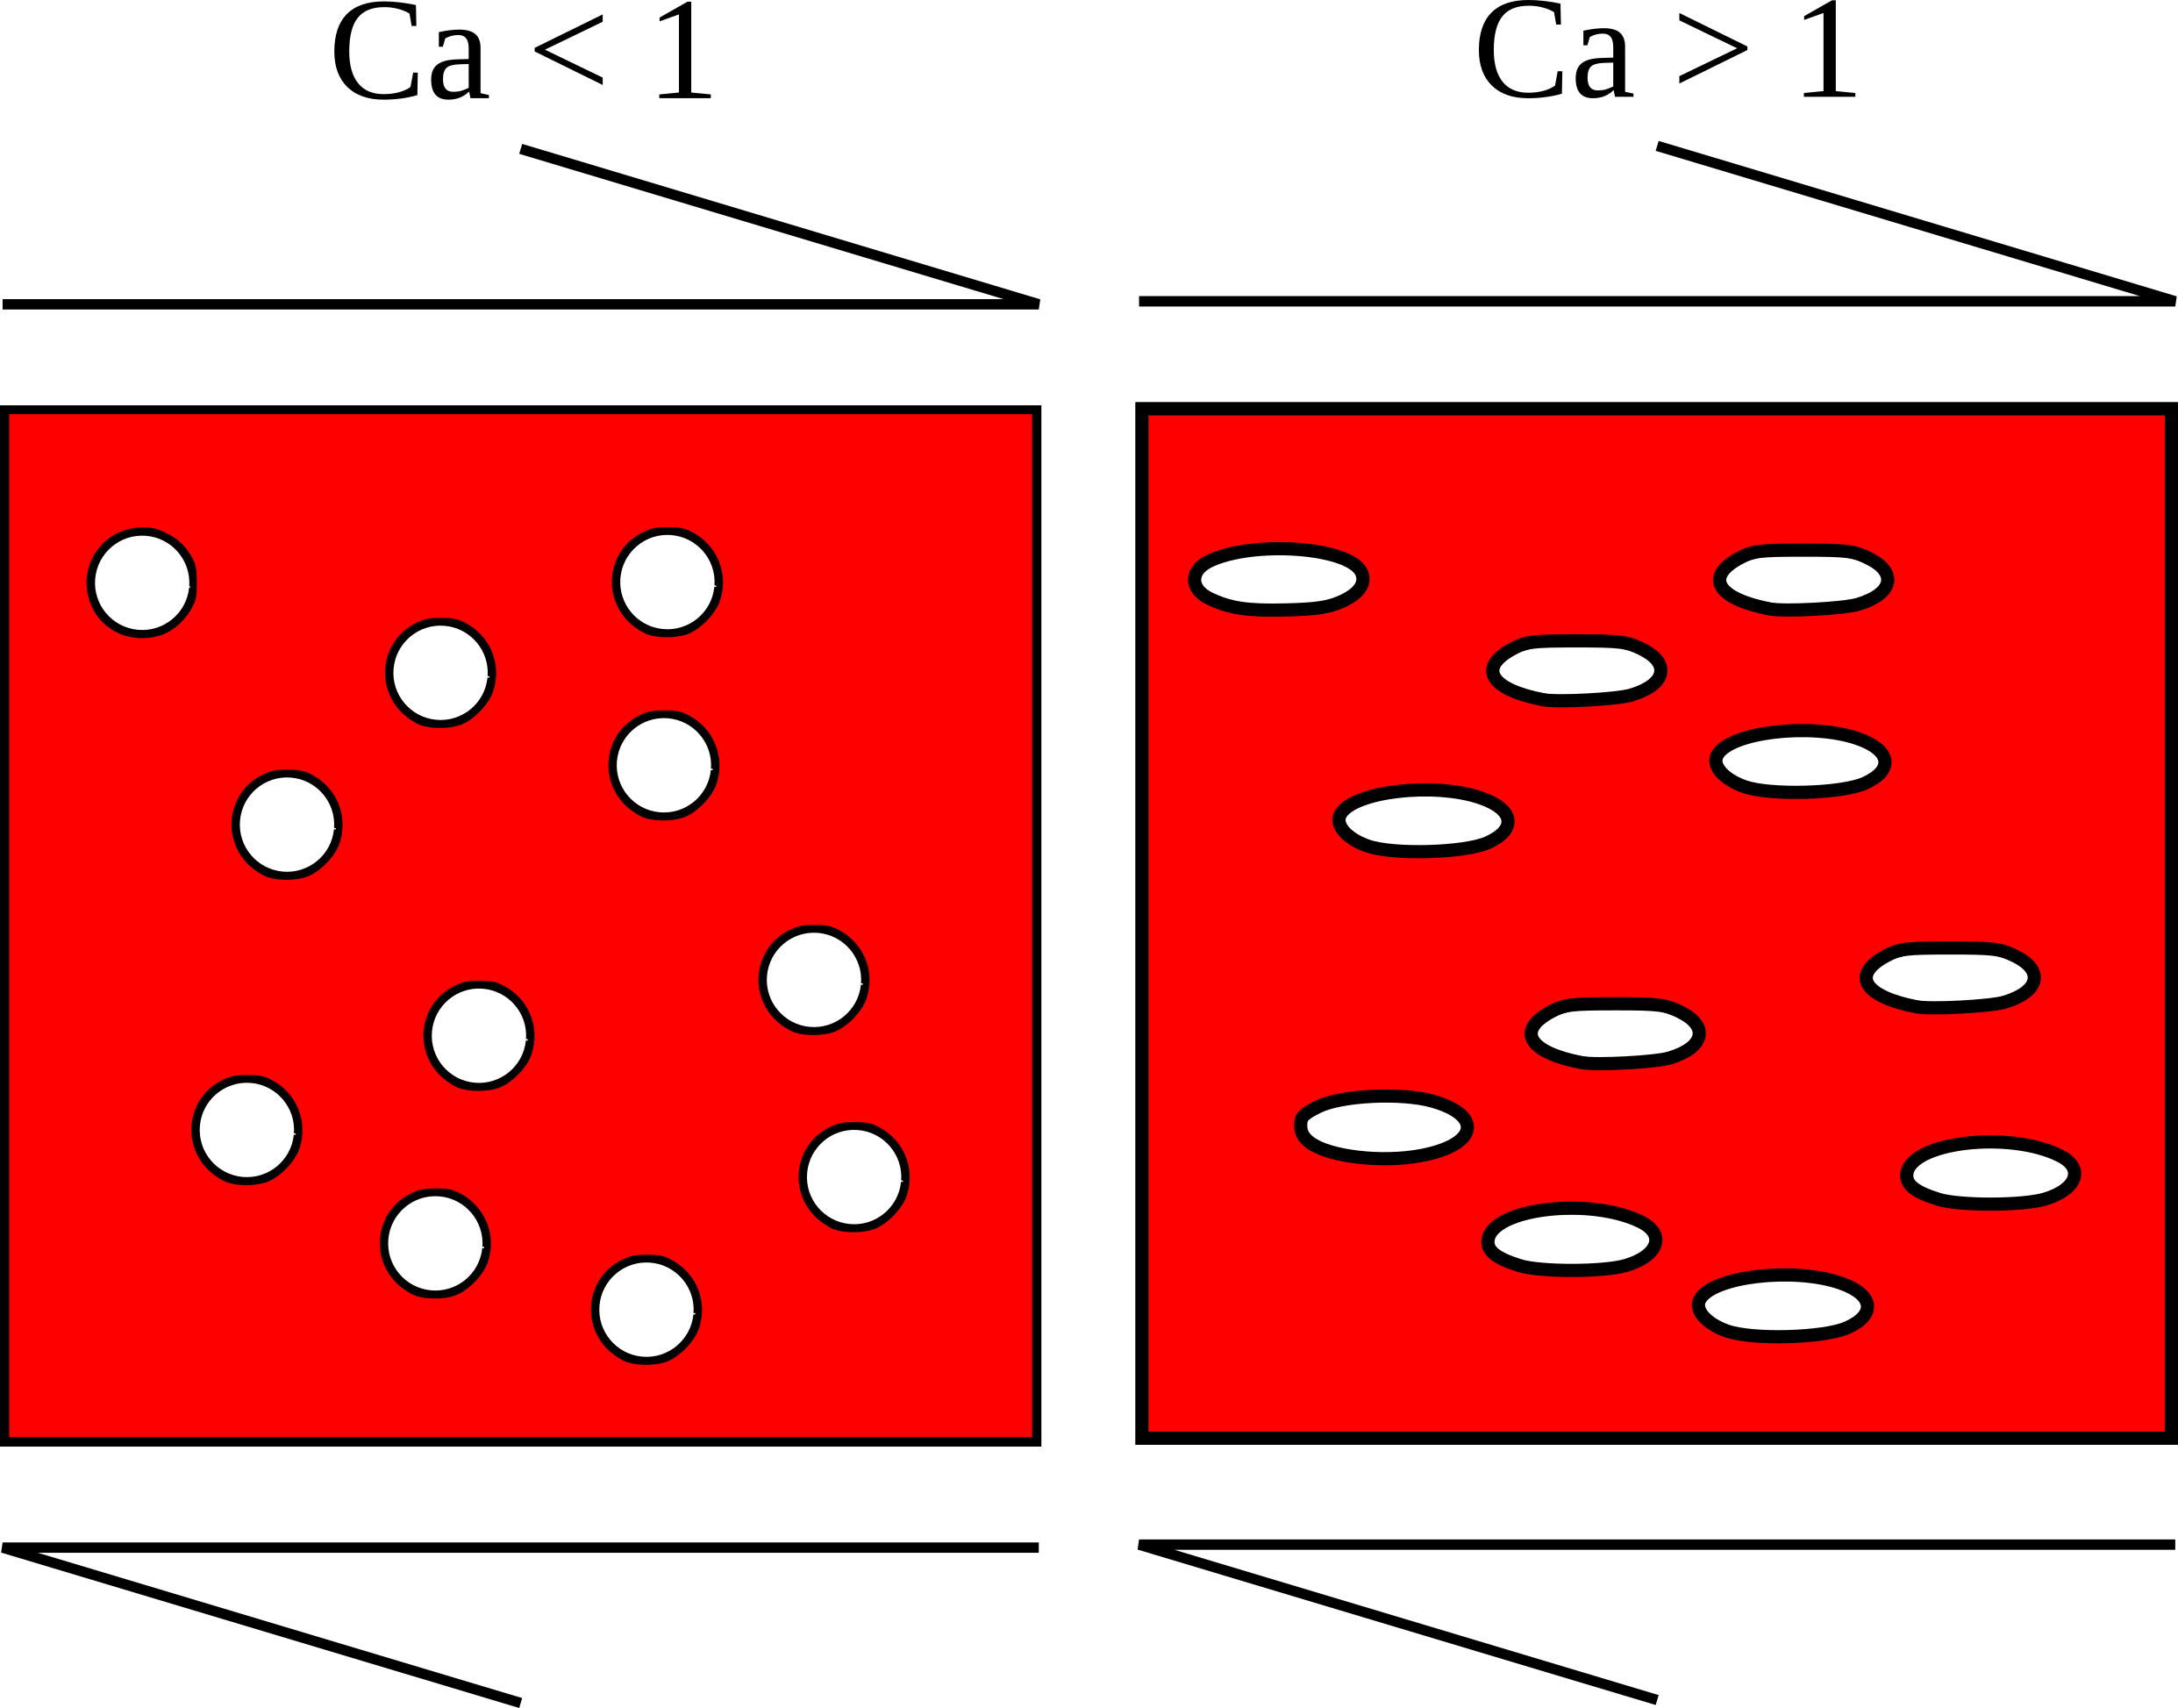
\includegraphics[width=0.9\textwidth]{capillary.png}$$

    \end{column}

    \begin{column}{0.5\textwidth}

      $\text{Ca}$ is a balance between:

      \begin{itemize}
      \item \textbf{Deforming viscous stress} $\eta_{\text{m}} \dot{\epsilon}$ \\
      \item \textbf{Restoring surface tension stress} $\sigma / r_{\text{b}}$ \\
      \end{itemize}

      \vspace{0.5cm}
      
      If $\text{Ca} \lesssim 1$, surface tension stress dominates and bubbles remain spherical \\
      \hspace*{0.5cm} Bubbles behave like solid particles \\
      \hspace*{1cm} $\implies$ increase in viscosity \\

      \vspace{0.5cm}
      
      If $\text{Ca} \gtrsim 1$, deforming stress dominates and bubbles can have irregular shapes \\
      \hspace*{0.5cm} Bubbles streamline with shear \\
      \hspace*{1cm} $\implies$ Decrease in viscosity and
      \hspace*{1.85cm} shear thinning \\

    \end{column}
    
  \end{columns}

\end{frame}
%------------------------------------------------
\begin{frame}
  \frametitle{Magma viscosity - Modeling the effect of bubbles}

  Bubble deformation makes it difficult to model effect of bubbles on rheology \\

  \vspace{0.5cm}
  
  \textbf{Relaxation time} - Characteristic time for a deformed bubble to return to equilibrium state \\

  $$ \lambda = \frac{\eta_{\text{m}} r_{\text{b}}}{\sigma} $$

  Compare with timescale for changing shear conditions $\dot{\gamma}/\ddot{\gamma}$

  \vspace{0.5cm}
  
  Define \textbf{Dynamic capillary number:}

  $$ \text{Cd} = \frac{\lambda \ddot{\gamma}}{\dot{\gamma}} $$

  $\text{Cd} < 1 \implies$ Steady flow \hspace{0.25cm} $\implies$ Rheology controlled by $\text{Ca}$ \\

  $\text{Cd} > 1 \implies$ Unsteady flow $\implies$ Bubbles never in equilibrium \\

  \hspace{5.5cm} Viscosity is less than bubble-free fluid \\
  
\end{frame}
%------------------------------------------------
\begin{frame}
  \frametitle{Magma viscosity - Modeling the effect of bubbles}

  Whether bubbles increase or decrease viscosity depends on $\dot{\gamma}$ and $\ddot{\gamma}$ \\

  Semi-empirical model of Mader et al. (2013):
  
  \begin{columns}[t]

    \begin{column}{0.5\paperwidth}

      $$ \eta_{\text{r}} = \eta_{\text{r}, \infty} + \frac{\eta_{\text{r}, 0} - \eta_{\text{r}, \infty}}{1 + \text{Cx}^{m}} $$

      where

      $$ \eta_{\text{r}, \infty} = 1 - \frac{5 \phi_{\text{b}}}{3} $$

      $$ \eta_{\text{r}, 0} = 1 + \phi_{\text{b}} $$
      
      $$ \text{Cx} = \sqrt{\text{Ca}^{2} + \text{Cd}^{2}} $$

      $m$ depends on size distribution \\

      \hspace{0.3cm} = 2 for mono-disperse bubbles \\
      
    \end{column}

    \begin{column}{0.5\paperwidth}

      $$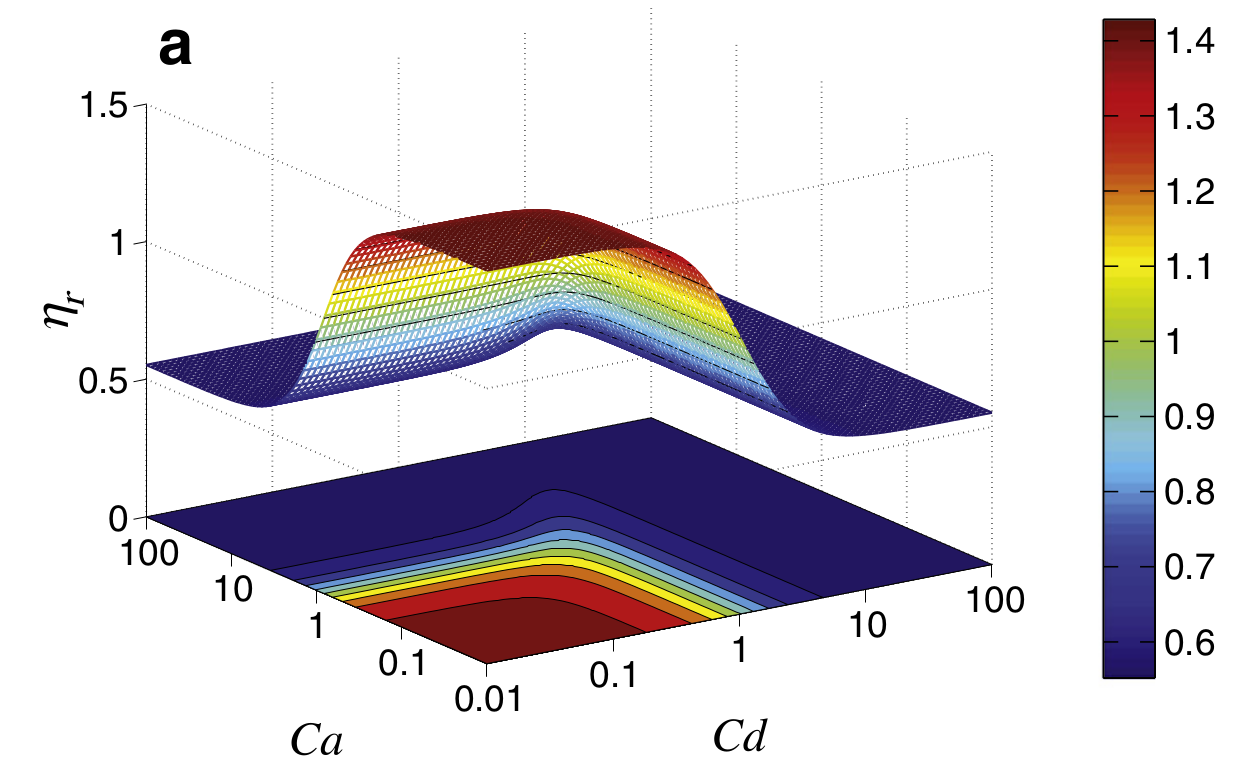
\includegraphics[width=0.9\textwidth]{Mader13.png}$$

      \vspace{-0.2cm}

      \centering \tiny Mader et al. (2013)

      \normalsize Experimentally tested for $\phi_{\text{b}} < 0.46$ \\

      \vspace{0.5cm}
      
      For $\phi_{\text{b}} \geq 0.74$ a foam forms \\
    \end{column}

  \end{columns}
\end{frame}
%------------------------------------------------

\begin{frame}
  \frametitle{Magma density and viscosity - conclusions}

  \begin{itemize}
  \item Empirical and semi-empirical models parameterise magma density and viscosity \\
    \vspace{0.5cm}
  \item Both depend on volume fraction of solid and gas phases \\
    \vspace{0.5cm}
  \item Melt density is described by an empirical equation of state and depends strongly on water content \\
    \vspace{0.5cm}
  \item Melt viscosity is described by an empirical VFT equation and depends on temperature and composition \\
    \vspace{0.5cm}
  \item Magma viscosity strongly depends on crystal and bubble content \\
  \end{itemize}
\end{frame}
%------------------------------------------------


\end{document}
